\documentclass[11pt]{article}

% ------------------------------------------------------------------
% Packages
% ------------------------------------------------------------------
\usepackage[utf8]{inputenc}
\usepackage[T1]{fontenc}
\usepackage{amsmath,amssymb,amsthm}
\usepackage{graphicx}
\usepackage{booktabs}
\usepackage{geometry}
\usepackage{hyperref}
\usepackage{natbib}
\usepackage{xcolor}
\usepackage{subcaption}
\usepackage{microtype}

\geometry{margin=1in}
\hypersetup{colorlinks=true, linkcolor=blue, citecolor=blue, urlcolor=blue}

\newcommand{\Pcal}{\mathcal{P}}
\newcommand{\Dcal}{\mathcal{D}}
\newcommand{\Xcal}{\mathcal{X}}
\newcommand{\Ycal}{\mathcal{Y}}
\newcommand{\TODO}[1]{\textcolor{red}{[TODO: #1]}}

\title{Conformal False Discovery Rate Control for Molecular\\
Property Prediction Under Covariate Shift}

\author{Maximilian Beckers}
\date{\today}

\begin{document}
\sloppy

\maketitle

\begin{abstract}
Virtual screening requires selecting a subset of compounds predicted
to satisfy a property threshold (e.g., sufficient solubility, permeability, or
metabolic stability) from a much larger,  unlabelled library.  Because thousands of
compounds are tested simultaneously, naive thresholding of a regression or
classification score inflates the false discovery rate (FDR) among the selected
set, and the miscalibration is compounded when the model is applied to compounds
that are structurally dissimilar from the calibration data --- the norm rather than
the exception in prospective screening. We introduce a conformal hypothesis-testing
framework for this setting: for each candidate compound we test the null hypothesis
that its property value does not exceed a decision threshold $\tau$,  and compute an
exact,  finite-sample-valid p-value against an empirical null distribution formed
from the negative (sub-threshold) subset of an independent calibration set. To adjust for distribution shift, we further introduce three importance-weighting schemes ---
entropy balancing, direct Kolmogorov--Smirnov (KS) distance minimisation, and local
Tanimoto-similarity (k-nearest-neighbour) weighting --- that re-weight the
calibration set so that its Morgan-fingerprint neighbour-distance distribution
matches that of the target (test) compounds, restoring approximate exchangeability
under scaffold- or cluster-induced covariate shift. We evaluate the framework on real ADMET endpoints (Caco-2 permeability, human liver microsomal intrinsic
clearance, and kinetic solubility) under random, cluster-based, and scaffold-based
splits, on a 100-assay ChEMBL bioactivity benchmark, and on a synthetic scaffold
R-group enumeration designed to isolate covariate shift from all other confounders.
Unweighted conformal FDR control is reliable under random splits but degrades
substantially under structural splits, with median true FDR exceeding the nominal
level for the majority of assays under cluster-based splitting. Importance
weighting reduces this violation, at the cost of a smaller, more conservative
selected set when the shift is severe.
\end{abstract}

% ==================================================================
\section{Introduction}
% ==================================================================

Machine learning models for molecular property prediction --- solubility,
permeability, metabolic stability, target potency --- are typically deployed to
screen tens of thousands to millions of virtual compounds and return a shortlist
for synthesis. This is fundamentally a multiple-hypothesis-testing problem: each
compound in the library corresponds to one hypothesis test of whether its true
property value crosses a decision threshold, and the fraction of false positives
in the returned shortlist (the false discovery rate, FDR) is the quantity a
practitioner actually cares about, not the pointwise accuracy of the underlying
regression or classification model. Reporting a raw model score, or even a
well-calibrated probability, does not by itself control the FDR of a shortlist
selected at some cutoff, because that guarantee requires accounting for the
number of hypotheses tested and the correlation structure between them
\citep{benjamini1995}.

Conformal prediction offers a route to distribution-free, finite-sample-valid
p-values without parametric assumptions on the model's error distribution
\citep{vovk2005,shafer2008}, and recent work has shown how to turn conformal
p-values into FDR-controlling procedures via the Benjamini--Hochberg (BH)
procedure, both for outlier/novelty detection \citep{bates2023} and for
selection problems more broadly \citep{jin2023selection}. All of these
guarantees, however, rest on an exchangeability assumption between the
calibration data and the test point. In molecular property prediction this
assumption is routinely violated by design: the very purpose of a model is to
extrapolate to new chemical series, and reliable retrospective evaluation of a
model in drug discovery requires scaffold- or cluster-based splitting precisely
because random splits over-estimate performance on future, structurally novel
compounds \citep{martin2017,schiebroek2026}. A calibration set built from
already-synthesized chemical matter is therefore systematically closer to
itself, in fingerprint space, than to the virtual library a model will actually
be asked to triage --- a covariate shift that can silently break the validity of
a naively BH-adjusted conformal p-value.

This paper develops and empirically stress-tests a conformal FDR-control
framework for this setting. Concretely, we:
\begin{enumerate}
    \item formalise molecular threshold screening as a one-sided hypothesis test
    per compound and define a \emph{Subpopulation Prediction Distribution Test}
    (SPDT) that calibrates against the model's predictions on the
    sub-threshold subpopulation only, rather than against a global residual
    distribution (Section~\ref{sec:methods});
    \item extend this test with three importance-weighting schemes --- entropy
    balancing, KS-distance minimisation, and local Tanimoto k-NN weighting ---
    that correct for covariate shift between calibration and target compounds
    by re-weighting the calibration set in fingerprint neighbour-distance space
    (Section~\ref{sec:weighting});
    \item quantify, on three ADMET endpoints, a 100-assay ChEMBL bioactivity
    benchmark, and a controlled synthetic scaffold-swap experiment, how badly
    naive (unweighted) conformal FDR control is violated under scaffold- and
    cluster-based splits, and to what extent importance weighting restores
    nominal control (Section~\ref{sec:experiments}--\ref{sec:results}).
\end{enumerate}

\paragraph{Scope of this draft.} This document is an initial, code-grounded
draft assembled directly from the accompanying implementation
(\texttt{src/conformal\_predictor.py}, \texttt{src/train\_xgboost.py},
\texttt{src/train\_xgboost\_schiebroek.py}, \texttt{src/scaffold\_experiment\_1.py})
and the result artefacts already produced (\texttt{results/*.csv},
\texttt{results/*.pkl}). Numbers reported in Section~\ref{sec:results} are
computed from those artefacts; sections marked \TODO{} indicate analyses the
code supports but for which results have not yet been generated or written up.

% ==================================================================
\section{Related Work}
% ==================================================================

\paragraph{Conformal prediction and weighted exchangeability.}
Conformal prediction \citep{vovk2005} converts any model score into
finite-sample-valid p-values or prediction sets under the sole assumption of
exchangeability between calibration and test data. \citet{tibshirani2019}
extend the framework to \emph{covariate shift}, showing that replacing uniform
calibration weights with likelihood-ratio importance weights restores validity
when the test covariate distribution differs from the calibration
distribution but the two share a common conditional law of $Y \mid X$. Our
weighting schemes are practical, density-ratio-free instantiations of this
idea, using nearest-neighbour Tanimoto distance in fingerprint space as a
proxy for the unknown likelihood ratio.

\paragraph{Conformal p-values, outlier testing, and FDR control.}
\citet{bates2023} introduce conformal p-values for testing whether a new
point is an outlier relative to an inlier calibration set, and show that
Benjamini--Hochberg applied to these p-values controls the FDR among
flagged outliers. Our setting differs in target and structure
(Section~\ref{sec:spdt-vs-outlier}): we test a directed hypothesis about a
continuous, \emph{labelled} response variable rather than performing
unsupervised out-of-distribution detection, and our empirical null is built
from the model's own predictions on a labelled sub-threshold subpopulation
rather than from a generic conformity score over the feature space. The
underlying multiple-testing machinery --- Benjamini--Hochberg \citep{benjamini1995},
Benjamini--Yekutieli for arbitrary dependence \citep{benjamini2001}, and the
Holm and Hochberg step-down/step-up procedures for family-wise error control
\citep{holm1979,hochberg1988} --- is standard and implemented directly
(\texttt{ConformalPredictor.p\_adjust}).

\paragraph{Risk-controlling prediction and selective inference.}
Risk-controlling prediction sets (RCPS; \citealp{bates2021}) calibrate a
single global threshold so that a user-specified risk (e.g., expected loss) is
controlled in expectation over the population; the closely related conformal
risk control framework \citep{angelopoulos2023} generalises this to a broad
class of monotone risks. These frameworks calibrate a \emph{global} error
distribution $|Y-\hat Y|$ over the full population, which can be
mis-calibrated under heteroskedastic error or population-dependent bias.
SPDT instead conditions calibration on the sub-threshold subpopulation
specifically, trading generality for a null distribution that mirrors the
model's actual behaviour on definitionally-negative compounds.

\paragraph{Distribution shift in molecular machine learning.}
It is well established that random train/test splits over-estimate
prospective model performance in drug discovery, and that scaffold- or
cluster-based splits are a more faithful proxy for deployment on novel
chemical series \citep{martin2017,wu2018moleculenet}. We adopt the
cluster-based (Butina) splitting protocol of \citet{schiebroek2026} for the
ChEMBL bioactivity benchmark (Section~\ref{sec:data-schiebroek}) and use the
resulting benchmark as the primary evidence that covariate shift, not merely
model miscalibration, is responsible for FDR violations under structural
splits.

% ==================================================================
\section{Methods}
\label{sec:methods}
% ==================================================================

\subsection{Problem formulation and the Subpopulation Prediction Distribution
Test (SPDT)}
\label{sec:spdt}

We consider a setting where each molecule $i$ is characterised by a feature
vector $X_i \in \Xcal$ (a Morgan fingerprint, optionally concatenated with
RDKit physicochemical descriptors) and a target property $Y_i$, which may be
continuous (e.g., $\log P$, intrinsic clearance) or binary (e.g., an
assay-specific active/inactive call). Let $f: \Xcal \to \mathbb{R}$ be a model
trained to predict $Y$ (or, in the classification case, the probability of the
positive class), yielding scores $\hat Y_i = f(X_i)$. The screening objective
is to act as an asymmetric filter: for a novel, unlabelled compound with
features $X_{\mathrm{new}}$ and unknown true property $Y_{\mathrm{new}}$, we
test the null hypothesis
\[
H_0 : Y_{\mathrm{new}} \le \tau ,
\]
where $\tau$ is a pre-specified decision threshold (e.g., $\tau = 200\,\mu M$
for kinetic solubility, or $\tau = 0.5$ on the predicted probability scale for
a classification endpoint). Rejecting $H_0$ corresponds to nominating the
compound for synthesis or follow-up.

To evaluate $H_0$ without parametric assumptions on the model's error
distribution, we use a \textbf{Subpopulation Prediction Distribution Test
(SPDT)}. Unlike standard conformal regression or risk-controlling prediction
sets \citep{bates2021}, which calibrate a global residual distribution
$|Y - \hat Y|$ over the whole calibration set, SPDT evaluates the raw
prediction $\hat Y_{\mathrm{new}}$ against an empirical null distribution
built exclusively from the sub-threshold (definitionally negative)
subpopulation.

\subsubsection{Calibration and empirical null distribution}

Let $\Dcal_{\mathrm{cal}} = \{(X_i, Y_i)\}_{i=1}^n$ be a calibration set
independent of the training data (in our experiments, a held-out validation
split). We construct the conditioned calibration subset
\[
\Dcal_{\mathrm{cal}}^{\le \tau} = \{(X_i, Y_i) \in \Dcal_{\mathrm{cal}} : Y_i \le \tau\},
\qquad m = \bigl|\Dcal_{\mathrm{cal}}^{\le \tau}\bigr|,
\]
and extract the corresponding model predictions to form the empirical null
pool
\[
\Pcal_0 = \{\hat Y_i : (X_i, Y_i) \in \Dcal_{\mathrm{cal}}^{\le \tau}\}.
\]
By conditioning on $Y_i \le \tau$, $\Pcal_0$ captures both the intrinsic
variance of the sub-threshold subpopulation and any systematic model bias
specific to that regime, sidestepping the need to model heteroskedasticity
across the full response range. We define the empirical CDF of $\Pcal_0$ as
\[
F_m(t) = \frac{1}{m}\sum_{\hat Y_i \in \Pcal_0} \mathbb{I}(\hat Y_i \le t).
\]

\subsubsection{Conformal p-value and decision rule}
\label{sec:pvalue}

Given a new compound with prediction $\hat Y_{\mathrm{new}} = f(X_{\mathrm{new}})$,
and assuming exchangeability between $\hat Y_{\mathrm{new}}$ and $\Pcal_0$
under $H_0$, the (uniformly weighted) conformal p-value is
\begin{equation}
p(X_{\mathrm{new}}) = \frac{1 + \sum_{\hat Y_i \in \Pcal_0} \mathbb{I}(\hat Y_i \ge \hat Y_{\mathrm{new}})}{m+1}.
\label{eq:pvalue-uniform}
\end{equation}
The $+1$ in numerator and denominator guarantees exact finite-sample validity:
under $H_0$ and exchangeability, $p(X_{\mathrm{new}})$ is super-uniform on
$[0,1]$. We reject $H_0$ at level $\alpha$ if $p(X_{\mathrm{new}}) \le \alpha$.
The implementation (\texttt{ConformalPredictor.predict\_pvalues}) generalises
this to importance-weighted calibration samples $w_i$ and an optional test
weight $w_{\mathrm{test}}$, following \citet{tibshirani2019}:
\[
p_j = \frac{\sum_i w_i\, \mathbb{I}(\alpha_i \ge \alpha_j) + w_{\mathrm{test},j}}
           {\sum_i w_i + w_{\mathrm{test},j}},
\label{eq:weighted-pvalue}
\]
where $\alpha$ denotes either the raw model score (SPDT, as above) or a
nonconformity score $Y_i - \hat Y_i$ computed over the \emph{full} calibration
set (Section~\ref{sec:pooling}); the indicator direction flips accordingly.
Uniform weights ($w_i \equiv 1$) recover Eq.~(\ref{eq:pvalue-uniform}) exactly.

\subsubsection{Two ways to pool calibration information}
\label{sec:pooling}

The implementation supports two calibration pools, both computed for every
dataset in Section~\ref{sec:results}:
\begin{itemize}
    \item \textbf{Score-based, negatives-only} (SPDT as defined above):
    calibration is restricted to $\Dcal_{\mathrm{cal}}^{\le\tau}$ and the
    conformity statistic is the raw model score $\hat Y_i$.
    \item \textbf{Nonconformity-based, all calibration points}: every
    calibration compound is used, with nonconformity score
    $V_i = Y_i - \hat Y_i$ for the true label and
    $V_{\mathrm{new}} = \tau - \hat Y_{\mathrm{new}}$ for the (unknown) test
    label evaluated at the null boundary
    (\texttt{ConformalPredictor.get\_nonconformity\_scores}). This uses the
    full calibration set, at the cost of a symmetric rather than
    one-sided nonconformity notion.
\end{itemize}
Both pools are combined with each of the three weighting schemes below,
giving six p-value variants per dataset/split.

\subsubsection{Multiple-hypothesis correction}

Applying the decision rule of Section~\ref{sec:pvalue} independently to every
compound in a virtual library of size $N$ controls only the per-compound Type-I
error; the expected fraction of false positives in the returned shortlist can
be far higher. We instead adjust the raw p-values $\{p_j\}_{j=1}^N$ with the
Benjamini--Hochberg (BH) procedure \citep{benjamini1995} to control the FDR at
level $q$ under the (weighted-)exchangeability guarantee of
Section~\ref{sec:pvalue}, and additionally provide Benjamini--Yekutieli (BY,
valid under arbitrary dependence; \citealp{benjamini2001}), Holm
\citep{holm1979}, and Hochberg \citep{hochberg1988} as more conservative
alternatives (\texttt{ConformalPredictor.p\_adjust}). A compound is selected
if its adjusted p-value is $\le q$.

\subsubsection{Distinct relation to conformal outlier testing}
\label{sec:spdt-vs-outlier}

SPDT should be distinguished from conformal p-values for outlier / novelty
detection, e.g.\ \citet{bates2023}. Both use the calibration-then-test
paradigm of conformal inference to produce non-parametric, FDR-controllable
p-values, but they differ in target and construction:
\begin{enumerate}
    \item \textbf{Target of inference.} \citet{bates2023} address unlabelled,
    unsupervised out-of-distribution testing: a model-agnostic conformity
    score over $\Xcal$ flags structural novelty. SPDT is a supervised,
    directed test that thresholds the continuous response space $\Ycal$,
    using $\Xcal$ only indirectly, through the model $f$ and (in the weighted
    variants) through covariate-shift correction.
    \item \textbf{Null construction.} Standard conformal regression relies on
    a global error distribution $|Y-\hat Y|$, which can be over- or
    under-conservative under heteroskedasticity. SPDT discards the
    above-threshold subpopulation entirely during calibration, so the test
    statistic is evaluated strictly against the model's empirical behaviour
    (local bias and variance) on valid (sub-threshold) structures.
\end{enumerate}

\subsection{Covariate shift and importance-weighted calibration}
\label{sec:weighting}

The validity argument in Section~\ref{sec:pvalue} requires
$(\hat Y_{\mathrm{new}}, \Pcal_0)$ to be (weighted-)exchangeable. When the test
compound is drawn from a different region of chemical space than the
calibration set --- the expected situation under scaffold- or cluster-based
splitting, and the realistic situation in prospective virtual screening ---
this assumption fails, because the calibration compounds nearest to
$X_{\mathrm{new}}$ in structure are systematically over- or under-represented
relative to a uniformly exchangeable draw. Following the weighted-conformal
framework of \citet{tibshirani2019}, we correct for this by replacing the
uniform calibration weights in Eq.~(\ref{eq:weighted-pvalue}) with importance
weights $w_i$ that approximate the covariate density ratio between the target
(test) and calibration (control) distributions. Because the true density
ratio over 2048-bit Morgan fingerprints is intractable, we approximate it
using the distribution of mean $k$-nearest-neighbour (Tanimoto) distances from
each calibration compound to the target set, and implement three schemes of
increasing locality (\texttt{src/conformal\_predictor.py}):

\paragraph{(i) Entropy balancing.} Let $X_i^{\mathrm{ctrl}}$ be the mean
5-NN Tanimoto distance from calibration compound $i$ to the (sub-sampled)
target set, and $X_j^{\mathrm{tgt}}$ the corresponding mean 5-NN distance of
target compound $j$ to the rest of the target set. We solve
\[
\max_{w \ge 0} \; -\sum_i w_i \log w_i
\quad \text{s.t.} \quad
\tfrac{1}{n}\textstyle\sum_i w_i = 1, \;\;
\mathrm{KS}\bigl(\{X_i^{\mathrm{ctrl}}\}, w;\, \{X_j^{\mathrm{tgt}}\}\bigr) \le \delta,
\]
where $\mathrm{KS}(\cdot,\cdot)$ is the weighted Kolmogorov--Smirnov distance
between the (re-weighted) empirical CDFs of the control and target
neighbour-distance distributions, and $\delta$ (\texttt{ks\_bound}) is a
user-set tolerance. This is a maximum-entropy formulation: among all weight
vectors that bring the two distributions within $\delta$ in KS distance, it
selects the one closest to uniform, minimising variance inflation. If the
unweighted KS distance is already $\le \delta$, weights are left uniform. The
optimisation is solved with SLSQP (\texttt{scipy.optimize.minimize}), with
calibration sets larger than 5000 sub-sampled for tractability and the
resulting weights interpolated back onto the full set by neighbour-distance
rank.

\paragraph{(ii) Direct KS minimisation.} Rather than bounding the KS distance
and maximising entropy, this variant directly minimises the KS distance
subject to a floor on the effective sample size (ESS),
$\mathrm{ESS}(w) = (\sum_i w_i)^2 / \sum_i w_i^2 \ge n_{\mathrm{eff}}$
(default $n_{\mathrm{eff}}=30$, set to $100$ in all experiments in
Section~\ref{sec:results}). This is more aggressive than entropy balancing ---
it will use all of the available ESS budget to reduce distributional
mismatch --- and correspondingly more prone to variance inflation from a small
number of highly up-weighted calibration compounds.

\paragraph{(iii) Local k-NN (Tanimoto) weighting.} Rather than a single global
weight vector, this scheme assigns \emph{per-test-compound} weights: for each
target compound $j$, its $k$ nearest calibration neighbours (Tanimoto
distance on Morgan fingerprints, $k = $ \texttt{num\_nn}, $-1$ meaning
"all") receive weight $\exp(-\gamma \cdot d_{\mathrm{Tanimoto}})$, renormalised
to sum to $k$; all other calibration compounds receive weight zero for that
test point. The bandwidth $\gamma$ interpolates between a uniform local
average ($\gamma=0$, $\mathrm{ESS}=k$) and single-nearest-neighbour weighting
($\gamma \to \infty$, $\mathrm{ESS}\to 1$). Rather than fixing $\gamma$ by
hand, we solve for the value that yields a target mean effective sample size
$n_{\mathrm{eff}}$ across all target compounds via Brent root-finding on the
(monotone) map $\gamma \mapsto \overline{\mathrm{ESS}}(\gamma)$
(\texttt{ConformalPredictor.\_set\_gamma\_by\_ess}).

All three schemes reduce to the unweighted SPDT of Section~\ref{sec:spdt}
when \texttt{weighted=False}, which we use throughout as the baseline against
which the effect of covariate-shift correction is measured.

% ==================================================================
\section{Data and Experimental Setup}
\label{sec:experiments}
% ==================================================================

We evaluate the framework in three settings of increasing control: (a) three
real single-endpoint ADMET benchmarks under three splitting strategies, (b) a
100-assay ChEMBL bioactivity benchmark reused from \citet{schiebroek2026}, and
(c) a synthetic scaffold-enumeration experiment in which the covariate shift
is fully controlled by construction.

\subsection{Splitting strategies}
For every dataset we compare three train/validation/test partitions
(\texttt{src/utils.py}), which differ only in how structurally close the
calibration (validation) and target (test) compounds are to one another and
to training:
\begin{itemize}
    \item \textbf{Random split}: i.i.d. partition; calibration and test are
    exchangeable by construction and serve as the sanity-check baseline.
    \item \textbf{Scaffold split}: compounds are grouped by Bemis--Murcko
    scaffold and whole scaffold groups are assigned to train/val/test, so
    test-set scaffolds do not appear in calibration.
    \item \textbf{Cluster (Butina) split}: Morgan fingerprints (radius 3,
    2048 bits) are clustered with the Butina algorithm at a Tanimoto distance
    threshold of 0.65 (0.30 for the ADMET data-prep pipeline), small clusters
    are merged into their nearest large-cluster centroid, and clusters are
    then assigned to train/val/test by descending size --- the protocol of
    \citet{schiebroek2026}, intended to produce a more aggressive and more
    realistic structural shift than scaffold splitting alone.
\end{itemize}

\subsection{ADMET single-endpoint benchmarks}
\label{sec:data-admet}
We use three physicochemical/ADMET endpoints (\texttt{data/expansion\_data\_prep\_with\_splits\_*.csv}):
Caco-2 cell permeability ($P_{\mathrm{app}}$ A$\to$B), human liver microsomal
intrinsic clearance (HLM CLint), and kinetic aqueous solubility (KSOL). Each
endpoint is binarised at an assay-specific decision threshold $\tau$ (e.g.
$\tau = 200\,\mu M$ for KSOL) and modelled as binary classification;
$\mathrm{conf\_threshold}=0.5$ on the predicted probability is used as the
null boundary for SPDT (\texttt{run\_conformal\_fdr},
\texttt{src/train\_xgboost.py}). Features are 2048-bit radius-2 Morgan
fingerprints concatenated with the full RDKit descriptor set; an XGBoost
classifier (\texttt{binary:logistic}, depth 6, 100 boosting rounds) is trained
on the training split of each endpoint/split combination. For every
endpoint/split we compute six BH-adjusted p-value variants: \{unweighted,
kNN-weighted, KS-weighted\} $\times$ \{negatives-only score-based, all-calibration
nonconformity-based\} (Section~\ref{sec:pooling}); $n_{\mathrm{eff}}=100$ for
all weighted variants.

\subsection{100-assay ChEMBL bioactivity benchmark}
\label{sec:data-schiebroek}
To obtain a large number of independent replicates of the shift-vs-no-shift
comparison, we reuse the ChEMBL bioactivity benchmark of
\citet{schiebroek2026} (\texttt{data/data\_ schiebroek\_2026/}): 100
target-assay pairs (pChEMBL activity thresholded at $\tau=7$, i.e.\ IC$_{50}$/K$_i$
$\le 100\,$nM $\Rightarrow$ active), each with its own random, scaffold, and
Butina-cluster split, giving 300 independent train/calibrate/test
experiments in total (\texttt{src/train\_xgboost\_schiebroek.py}). Because of
the number of assays, this benchmark is used only with the unweighted SPDT
baseline in the current codebase; it establishes how frequently and how
severely FDR control is violated under structural splits before any
covariate-shift correction is applied, and is the primary motivating result
of this paper (Section~\ref{sec:results-schiebroek}).

\subsection{Synthetic scaffold-swap experiment}
\label{sec:data-synthetic}
Real chemical datasets confound covariate shift with sample size, label
imbalance, and assay noise, all of which independently affect FDR control. To
isolate the effect of covariate shift, \texttt{src/scaffold\_experiment\_1.py}
constructs a fully synthetic benchmark: two scaffolds (a piperidine,
"Scaffold A", and a trisubstituted-benzene/triazine, "Scaffold B") are each
enumerated over an 18-member R-group library at three independently-varied
substitution positions via RDKit \texttt{molzip}, producing on the order of
$18^3$ candidate compounds per scaffold (fewer after de-duplication and
sanitisation failures). The binary label is $\mathrm{MolLogP} \ge 7$
(computed from RDKit descriptors on the enumerated structure, with
independent Gaussian noise added to each scaffold's logP to avoid a
degenerate, perfectly separable label). Scaffold A is over-represented in
training and calibration and \emph{absent from test}; Scaffold B is split
50\%/10\%/40\% into train/calibration/test, so the test set is drawn entirely
from a scaffold that is a small minority of the calibration set --- a
controlled analogue of a structural split, with a known ground-truth
covariate shift direction. This lets us directly check, by construction,
whether the importance weights recovered by KS- and kNN-weighting up-weight
the (correct) Scaffold-B calibration compounds relative to Scaffold A. \TODO{
Results from this experiment (weight distributions by scaffold, FDR curves
on the all-Scaffold-B test set) have been produced interactively in the
notebook but not yet exported to \texttt{results/}; re-run
\texttt{scaffold\_experiment\_1.py} (or \texttt{scaffold\_experiment\_2.py}
for the corresponding ablation) and save outputs before finalising this
section.}

% ==================================================================
\section{Results}
\label{sec:results}
% ==================================================================

\subsection{Naive conformal FDR control degrades under structural splits}
\label{sec:results-schiebroek}

Table~\ref{tab:schiebroek} summarises the unweighted SPDT baseline across the
100-assay ChEMBL benchmark (Section~\ref{sec:data-schiebroek}), at a nominal
FDR level $q=0.2$. Random splitting controls the FDR reliably: the mean true
FDR across assays with at least one selected compound is close to nominal, and
98\% of assays keep the true FDR at or below the target. Both structural
splits degrade this substantially. Scaffold splitting raises the mean true
FDR to 0.131 and drops the fraction of well-controlled assays to 86\%.
Butina cluster splitting --- the more aggressive structural shift --- is
markedly worse: mean true FDR rises to 0.358, nearly double the nominal
level, and only 37\% of assays keep the true FDR at or below $q=0.2$.
Figure~\ref{fig:schiebroek-box} shows the full distribution: under cluster
splitting the interquartile range of true FDR sits well above the nominal
target, indicating that the failure is systematic rather than driven by a
handful of outlier assays.

\begin{table}[t]
\centering
\caption{Unweighted SPDT, 100 ChEMBL bioactivity assays
(\texttt{results/schiebroek\_results\_*.csv}), nominal FDR $q=0.2$. ``Assays
w/ selection'' excludes assays where no compound was selected at $q=0.2$ (no
FDR is defined in that case). Mean true FDR and the fraction of well-controlled
assays are computed over that subset.}
\label{tab:schiebroek}
\resizebox{\textwidth}{!}{%
\begin{tabular}{lccccc}
\toprule
Split & Mean AUROC & Mean AUPRC & Assays w/ selection & Mean true FDR & Frac.\ true FDR $\le 0.2$ \\
\midrule
Random           & 0.885 & 0.840 & 86/100 & 0.095 & 0.98 \\
Scaffold         & 0.834 & 0.781 & 76/100 & 0.131 & 0.86 \\
Butina cluster   & 0.748 & 0.689 & 59/100 & 0.358 & 0.37 \\
\bottomrule
\end{tabular}%
}
\end{table}

\begin{figure}[t]
\centering
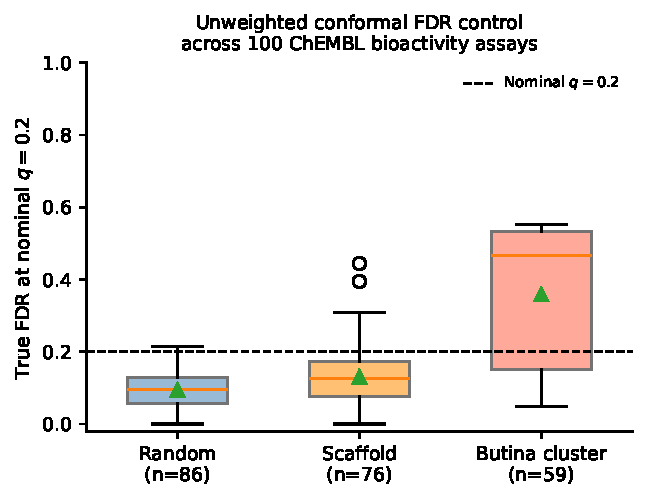
\includegraphics[width=0.5\textwidth]{paper_figures/fig_schiebroek_fdr_boxplot.pdf}
\caption{Distribution of true FDR at nominal $q=0.2$ across 100 ChEMBL
bioactivity assays, unweighted SPDT, by split type. Predictive performance
(mean AUROC) also degrades from random to scaffold to cluster splitting,
confirming that the cluster split induces a harder generalisation problem,
but the FDR-control failure is disproportionately larger than the AUROC
drop would suggest.}
\label{fig:schiebroek-box}
\end{figure}

Two observations motivate the weighting schemes of Section~\ref{sec:weighting}.
First, the ranking of split difficulty for FDR control (random $\ll$ scaffold
$\ll$ cluster) tracks the ranking of split difficulty for discrimination
(AUROC), consistent with structural shift being the common cause of both.
Second, the number of assays with \emph{zero} selected compounds at $q=0.2$
also rises sharply under cluster splitting (41/100, vs.\ 14/100 for random),
i.e.\ the unweighted procedure is simultaneously under-powered on many assays
and badly anti-conservative on others --- exactly the symptom expected when
exchangeability is violated non-uniformly across assays with different
degrees of scaffold overlap between calibration and test.

\subsection{Effect of importance weighting on ADMET endpoints}

Table~\ref{tab:admet} reports, for each ADMET endpoint and split, the number
of compounds selected at nominal FDR $q=0.2$ and the resulting true FDR, for
the unweighted, kNN-weighted, and KS-weighted score-based variants
(Section~\ref{sec:pooling}; the nonconformity-based variants selected zero
compounds in every configuration tested so far and are omitted --
\TODO{diagnose why the all-calibration nonconformity pooling is currently
over-conservative; likely the symmetric, two-sided nonconformity score is
too permissive as a null-distribution boundary for these class-imbalanced
endpoints, and needs either a one-sided nonconformity definition or a
less conservative $\tau$}).

\begin{table}[t]
\centering
\caption{ADMET endpoints, nominal FDR $q=0.2$, score-based SPDT
(\texttt{results/*\_fdr\_metrics.csv}). ``---'' indicates zero compounds
selected (true FDR undefined). All three splits use the same trained model
per endpoint; only the calibration/test partition differs.}
\label{tab:admet}
\resizebox{\textwidth}{!}{%
\begin{tabular}{llrrrrrr}
\toprule
& & \multicolumn{2}{c}{Unweighted} & \multicolumn{2}{c}{kNN-weighted} & \multicolumn{2}{c}{KS-weighted} \\
\cmidrule(lr){3-4}\cmidrule(lr){5-6}\cmidrule(lr){7-8}
Endpoint & Split & $n_{\mathrm{sel}}$ & FDR & $n_{\mathrm{sel}}$ & FDR & $n_{\mathrm{sel}}$ & FDR \\
\midrule
Caco-2 & Cluster   & 169 & 0.142 & 122 & 0.148 & 205 & 0.176 \\
Caco-2 & Scaffold  & 65  & 0.108 & 0   & ---   & 72  & 0.097 \\
HLM CLint & Random & 0   & ---   & 0   & ---   & 0   & ---   \\
HLM CLint & Cluster   & 0 & ---   & 0   & ---   & 0   & ---   \\
HLM CLint & Scaffold  & 0 & ---   & 0   & ---   & 0   & ---   \\
KSOL & Random    & 117 & 0.111 & 104 & 0.106 & 106 & 0.094 \\
KSOL & Cluster   & 34  & 0.088 & 19  & 0.000 & 40  & 0.075 \\
KSOL & Scaffold  & 26  & 0.077 & 23  & 0.087 & 46  & 0.065 \\
\bottomrule
\end{tabular}%
}
\end{table}

Two patterns stand out. First, unlike the 100-assay ChEMBL benchmark, all
three ADMET endpoints (where any compound is selected at all) show true FDR
\emph{below} the nominal $q=0.2$ for every method, weighted or not --- these
larger, more homogeneous single-endpoint datasets are evidently easier
exchangeability problems than the ChEMBL benchmark's smaller, more diverse
per-assay calibration sets. Second, where covariate shift is severe enough to
matter (KSOL under cluster and scaffold splitting), weighting has a
consistent, visible effect on the selected set size and, for KS-weighting,
on the true FDR (0.088 $\to$ 0.075 under cluster split; 0.077 $\to$ 0.065
under scaffold split), at the cost of being more conservative
(fewer compounds selected). The kNN-weighted variant is markedly more
conservative still, occasionally collapsing to zero selections under severe
shift (Caco-2, scaffold split) --- a direct consequence of the local
weighting scheme concentrating weight on very few effective calibration
neighbours (Section~\ref{sec:weighting}(iii)) when the target compounds are
structurally distant from all calibration compounds. HLM CLint selects zero
compounds under every method and split, most likely reflecting either a
poorly-separated classification boundary at the chosen threshold or too few
negative calibration examples surviving the $\mathrm{conf\_threshold}=0.5$
cut; \TODO{inspect the HLM CLint score distribution and negative-calibration
pool size directly (\texttt{scores\_calib\_neg} in the saved pickle) before
drawing conclusions from this endpoint}.

Figure~\ref{fig:ksol-fdr} shows the full FDR-control curve (true FDR as a
function of the nominal level, rather than the single value at $q=0.2$
tabulated above) for KSOL across all three splits. Under the random split
all three methods track the diagonal (nominal = true) closely at all
thresholds. Under the scaffold and cluster splits the unweighted curve
departs visibly from the diagonal at low nominal FDR, and both weighting
schemes pull the curve back toward calibration, most consistently for
KS-weighting.

\begin{figure}[t]
\centering
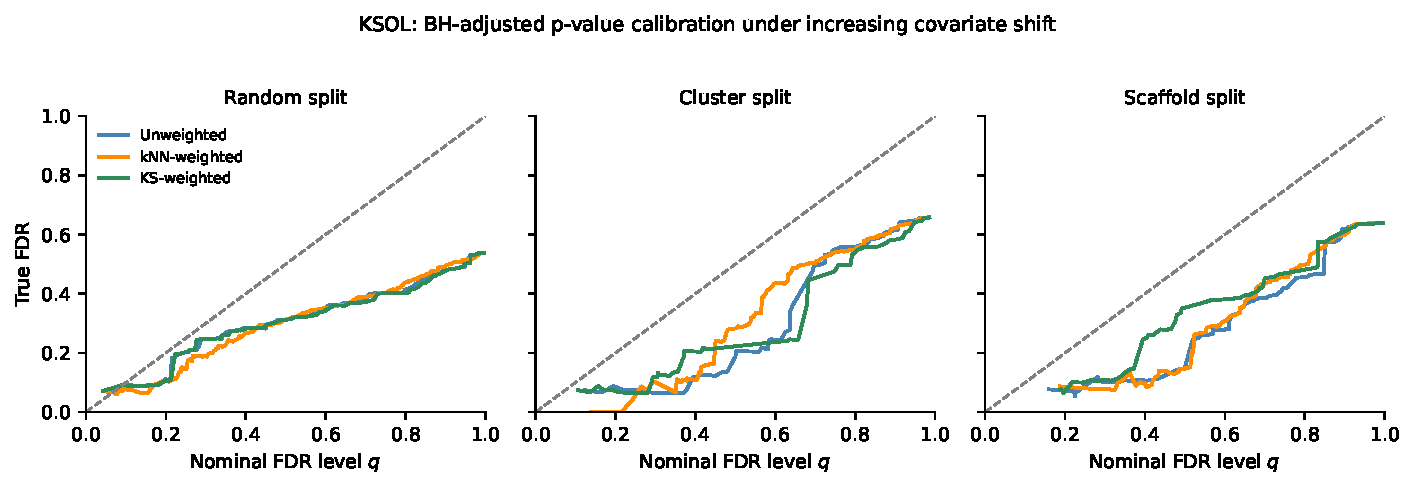
\includegraphics[width=\textwidth]{paper_figures/fig_ksol_fdr_curves.pdf}
\caption{KSOL: true FDR vs.\ nominal FDR level $q$, unweighted vs.\
kNN-weighted vs.\ KS-weighted SPDT, across random, cluster, and scaffold
splits. The diagonal is the target (true FDR = nominal FDR).}
\label{fig:ksol-fdr}
\end{figure}

Figure~\ref{fig:ksol-ecdf} illustrates the mechanism directly: under the KSOL
scaffold split, the empirical CDF of mean 5-NN Tanimoto distance (calibration
to target) sits well to the left of the corresponding target-to-target CDF
before weighting (calibration compounds are, on average, structurally closer
to other calibration compounds than target compounds are to each other,
reflecting a systematic proximity gap), and both weighting schemes shift the
weighted calibration CDF toward the target curve.

\begin{figure}[t]
\centering
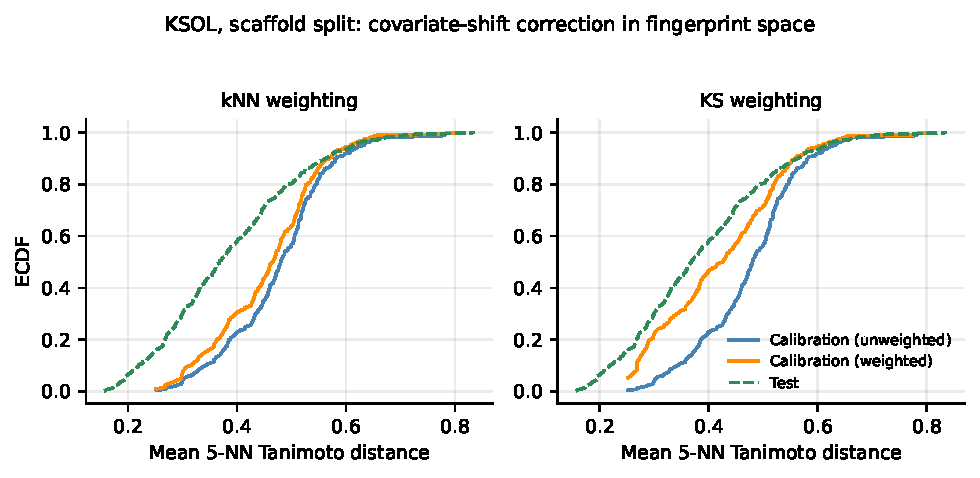
\includegraphics[width=0.75\textwidth]{paper_figures/fig_ksol_scaffold_ecdf.pdf}
\caption{KSOL, scaffold split: ECDF of mean 5-NN Tanimoto distance for the
calibration set before/after importance weighting, and for the target
(test) set, for kNN-weighting and KS-weighting. Bringing the weighted
calibration curve closer to the target curve is the explicit optimisation
objective of both schemes (Section~\ref{sec:weighting}).}
\label{fig:ksol-ecdf}
\end{figure}

\subsection{Synthetic scaffold-swap experiment}

\TODO{Pending re-run of \texttt{scaffold\_experiment\_1.py} with results
exported to \texttt{results/} (see Section~\ref{sec:data-synthetic}). This
section should report: (i) whether KS- and kNN-derived weights correctly
up-weight Scaffold-B calibration compounds relative to Scaffold A
(ground truth is known by construction here, unlike the real datasets); (ii)
the resulting FDR-control curve on the all-Scaffold-B test set, weighted vs.\
unweighted; and (iii) whether the direction and magnitude of the weighting
effect matches the real-data results in Table~\ref{tab:admet} and
Figure~\ref{fig:ksol-fdr}, as a sanity check that the real-data effect is
attributable to covariate shift specifically rather than a confound.}

% ==================================================================
\section{Discussion}
% ==================================================================

The central empirical finding is a dissociation between predictive
performance and FDR-control validity under structural splits. AUROC drops by
roughly 14 points from random to cluster splitting on the ChEMBL benchmark
(0.885 $\to$ 0.748), a meaningful but not catastrophic degradation by the
standards of prospective virtual screening; the true FDR at nominal $q=0.2$,
by contrast, nearly doubles (0.095 $\to$ 0.358), and the fraction of assays
with valid control collapses from 98\% to 37\%. A practitioner monitoring
only discrimination metrics would substantially under-estimate how
unreliable a naive FDR-controlled shortlist becomes under exactly the kind of
structural extrapolation that virtual screening exists to perform. This is
the practical case for covariate-shift-aware calibration, independent of any
improvement (or lack thereof) in the underlying predictive model.

The weighting schemes evaluated here provide partial, not complete,
correction, and exhibit a clear conservativeness/power trade-off: KS-weighting
consistently reduces true FDR at some cost in selected-set size, while local
kNN-weighting is considerably more aggressive about that trade-off and can
collapse to no selections under severe shift. This matches the theoretical
expectation that importance weighting trades type-I error control for reduced
effective sample size, and suggests KS-weighting (which optimises a single
global weight vector against an explicit ESS floor) as the more practically
useful default of the two importance-weighting schemes, with entropy
balancing (Section~\ref{sec:weighting}(i), not yet included in the tabulated
comparison --- \TODO{add entropy-balancing columns to Table~\ref{tab:admet};
the predictor class supports it but \texttt{run\_conformal\_fdr} in
\texttt{train\_xgboost.py} does not currently call it}) as a potentially
less variance-inflating alternative worth comparing directly.

The ChEMBL benchmark's zero-selection assays (41/100 under cluster
splitting) deserve more attention than a single aggregate true-FDR number
gives them: an assay that never crosses the selection threshold is not a
failure of \emph{validity} (no false discoveries are possible in an empty
set) but is a failure of \emph{power}, and a full account of the
weighting schemes' effect on this benchmark requires re-running it with
weighting enabled and reporting the joint distribution of power and
validity, not validity alone. \TODO{This is the single highest-priority
next experiment: currently \texttt{train\_xgboost\_schiebroek.py} only
computes the unweighted baseline; extending it to also compute
KS-/kNN-weighted p-values per assay, as already done for the ADMET
endpoints in \texttt{train\_xgboost.py}, would let
Table~\ref{tab:schiebroek} and Table~\ref{tab:admet} be compared on equal
footing.}

\paragraph{Limitations.} All weighting schemes here rely on nearest-neighbour
Tanimoto distance in Morgan-fingerprint space as a proxy for the true
covariate density ratio; this is a reasonable but crude surrogate, and its
adequacy has not been directly validated against a setting with a known
ground-truth density ratio other than the synthetic scaffold-swap experiment
(Section~\ref{sec:data-synthetic}, results pending). The single-endpoint
ADMET results (Table~\ref{tab:admet}) are each a single train/calibrate/test
realisation per split, with no resampling or confidence interval on the
reported true FDR; the 100-assay ChEMBL benchmark is the more statistically
reliable evidence for this reason, and future revisions of this paper should
either bootstrap the ADMET splits or otherwise report uncertainty on
Table~\ref{tab:admet}'s single-realisation FDR estimates.

% ==================================================================
\section{Conclusion}
% ==================================================================

We formalised molecular property screening as a large-scale, one-sided
hypothesis-testing problem and introduced a conformal FDR-control procedure
(SPDT) calibrated against the model's predictions on a labelled sub-threshold
subpopulation. We showed, on a 100-assay ChEMBL bioactivity benchmark, that
naive (unweighted) conformal FDR control is reliable under random splitting
but degrades sharply under scaffold- and especially cluster-based splitting
--- the splitting regimes that best approximate genuine prospective virtual
screening. We introduced three importance-weighting schemes that use
molecular-fingerprint neighbour-distance distributions to approximate the
covariate density ratio between calibration and target compounds, and showed
that at least one of them (KS-distance minimisation) measurably reduces true
FDR under structural shift on real ADMET data, at a cost in selected-set
size. Completing the weighted evaluation of the 100-assay benchmark and the
synthetic scaffold-swap experiment (Sections~\ref{sec:results-schiebroek},
\ref{sec:data-synthetic}) are the immediate next steps toward a full
account of when, and by how much, covariate-shift-aware conformal
calibration is worth its cost in statistical power.

% ==================================================================
\bibliographystyle{plainnat}
\begin{thebibliography}{99}

\bibitem[Angelopoulos et al.(2023)]{angelopoulos2023}
Angelopoulos, A.~N., Bates, S., Fisch, A., Lei, L., and Schuster, T. (2023).
Conformal risk control. \emph{arXiv preprint arXiv:2208.02814}.

\bibitem[Bates et al.(2021)]{bates2021}
Bates, S., Angelopoulos, A., Lei, L., Malik, J., and Jordan, M. (2021).
Distribution-free, risk-controlling prediction sets.
\emph{Journal of the ACM}, 68(6):1--34.

\bibitem[Bates et al.(2023)]{bates2023}
Bates, S., Cand\`es, E., Lei, L., Romano, Y., and Sesia, M. (2023).
Testing for outliers with conformal p-values.
\emph{The Annals of Statistics}, 51(1):149--178.

\bibitem[Benjamini and Hochberg(1995)]{benjamini1995}
Benjamini, Y. and Hochberg, Y. (1995).
Controlling the false discovery rate: a practical and powerful approach to
multiple testing. \emph{Journal of the Royal Statistical Society: Series B},
57(1):289--300.

\bibitem[Benjamini and Yekutieli(2001)]{benjamini2001}
Benjamini, Y. and Yekutieli, D. (2001).
The control of the false discovery rate in multiple testing under
dependency. \emph{The Annals of Statistics}, 29(4):1165--1188.

\bibitem[Hochberg(1988)]{hochberg1988}
Hochberg, Y. (1988).
A sharper Bonferroni procedure for multiple tests of significance.
\emph{Biometrika}, 75(4):800--802.

\bibitem[Holm(1979)]{holm1979}
Holm, S. (1979).
A simple sequentially rejective multiple test procedure.
\emph{Scandinavian Journal of Statistics}, 6(2):65--70.

\bibitem[Jin and Cand\`es(2023)]{jin2023selection}
Jin, Y. and Cand\`es, E.~J. (2023).
Model-free selective inference under covariate shift via weighted conformal
p-values. \emph{arXiv preprint arXiv:2307.09291}.

\bibitem[Martin et al.(2017)]{martin2017}
Martin, E.~J., Polyakov, V.~R., Tian, L., and Perez, R.~C. (2017).
Profile-QSAR 2.0: kinase virtual screening accuracy comparison across
methods and datasets. \emph{Journal of Chemical Information and Modeling},
57(8):2077--2088.

\bibitem[Schiebroek et al.(2026)]{schiebroek2026}
Schiebroek, C.~C.~G. et al. (2026).
\emph{[Full citation pending --- benchmark and cluster-based (Butina)
splitting protocol reused in \texttt{src/train\_xgboost\_schiebroek.py} and
\texttt{src/utils.py:cluster\_based\_split}.]}

\bibitem[Shafer and Vovk(2008)]{shafer2008}
Shafer, G. and Vovk, V. (2008).
A tutorial on conformal prediction.
\emph{Journal of Machine Learning Research}, 9:371--421.

\bibitem[Tibshirani et al.(2019)]{tibshirani2019}
Tibshirani, R.~J., Foygel Barber, R., Cand\`es, E.~J., and Ramdas, A. (2019).
Conformal prediction under covariate shift.
In \emph{Advances in Neural Information Processing Systems}, 32.

\bibitem[Vovk et al.(2005)]{vovk2005}
Vovk, V., Gammerman, A., and Shafer, G. (2005).
\emph{Algorithmic Learning in a Random World}. Springer.

\bibitem[Wu et al.(2018)]{wu2018moleculenet}
Wu, Z., Ramsundar, B., Feinberg, E.~N., Gomes, J., Geniesse, C., Pappu, A.~S.,
Leswing, K., and Pande, V. (2018).
MoleculeNet: a benchmark for molecular machine learning.
\emph{Chemical Science}, 9(2):513--530.

\end{thebibliography}

\end{document}
